\chapter{Machine learning for GPS clock prediction}


%====================================================================================================
\section{GPS clock adjusment}

%----------------------------------------------------------------------------------------------------
\subsection{Satellite and reference clocks}

%----------------------------------------------------------------------------------------------------
\subsection{Satellite brodcasted polynomial}
Currently every GPS device is able to calculate satellite clock bias based on
%TODO: Algorithm is configuring not message
parameters broadcasted in navigation message by the satellite itself which 
configure a second-degree polynomial:
\begin{equation}
	\Delta t_{sv}=a_{f0}+a_{f1}(t-t_{ref})+a_{f2}(t-t_{ref})^2+\Delta t,
\end{equation}
where $a_{f0}$, $a_{f1}$ and $a_{f2}$ are parameters sent in a satellite message, $t$ is GPS
time and $t_{ref}$ is a reference time. 
$\Delta t$ is the periodical component of a relativistic correction which is caused by 
gravitational field of earth and by a speed at which satellite orbits the planet.
This component is dependent on the orbit eccentricity and can be described as a:
\begin{equation}
 \Delta t=- 2\, \frac{\mathbf{r}_s \cdot \mathbf{v}_s}{c^2} \qquad,
\end{equation}
where $ {\mathbf r}_s$ and ${\mathbf v}_s$ are the satellite 
%TODO: Write more eloquently about units.
position ($\displaystyle m$) and velocity ($\displaystyle m/s$) vectors in an inertial system. 
While this method allows real-time corrections its precision is at the range of
nanoseconds \cite{Misra2011}, which results in an error of about 30 cm in localization calculation.
While this may be acceptable in-car navigation, robotic solutions require more precision that in
turn requires clock correction on the level of picoseconds.
Such corrections used along with proper measurement processing algorithm,
like Precise Point Positioning algorithm (PPP), will allow real-time or quasi-real-time localization with 
precision in the range of single centimeters\cite{krzan2015}.

%----------------------------------------------------------------------------------------------------
\subsection{IGU products}
The most widely used source of precise clock corrections are products provided 
by International GNSS Service (IGS) \cite{IGS}.
% TODO:Fix table size so it is not wider than text
\begin{table}[H] 
	\centering
	\caption{Variants of IGS products}
	\label{tab:igs_products}
	\begin{tabular*}{\textwidth}{*{5}{l}}
		\hline
		\hline
		Type& Accuracy& Latency& Update& Sample \\
		&&&&interval\\
		\hline
		Transmitted & 5ns & real time & -- & daily  \\
		Ultra rapid -- predicted & 3ns & real time & at 03, 09, 15, 21 UTC & 15 min  \\
		Ultra rapid -- observed & 150ps & 3-9 hours & at 03, 09, 15, 21 UTC & 15 min  \\
		Rapid & 75ps & 17-41 hours & at 17 UTC daily & 5 min \\
		Final & 75ps & 12-18 days & every Thursday & 30 s \\
		\hline
		\hline
	\end{tabular*}
\end{table}
Values shown in Table \ref{tab:igs_products} refer to satellite clock bias only,  IGS products
provide other information which full description  is available at  
\texttt{http://www.igs.org/products}.
IGS products can be easily divided into two categories:
\begin{itemize}
	\item real time consisting of transmitted and ultra rapid predicted half,
	\item high latency consisting of ultra rapid observed half as well as rapid and final products.
\end{itemize}
Solutions that have high latency are not usable in real-time navigation and as such will not be
considered in this work. Ultra-rapid observed part will be used as a source of
reference time so that if a bias prediction error is equal to zero it means that is
the same as provided by Ultra-rapid observed.
As can be seen in the Table \ref{tab:igs_products} all real-time solutions provide precision 
at a range of nanoseconds, aim of this work is to show that LSTM networks can provide 
better results than those solutions while still working at real-time response latency.

%====================================================================================================
\section{Classic ML approaches}

%----------------------------------------------------------------------------------------------------
\subsection{Polynomial regression}

%----------------------------------------------------------------------------------------------------
\subsection{Frequency analysis and reconstruction}

%----------------------------------------------------------------------------------------------------
\subsection{Adaptive filtering}


%====================================================================================================
\section{LSTM neural nerworks}

%----------------------------------------------------------------------------------------------------
\subsection{Research overwiev}
\paragraph{Machine learning pipeline}
In the project, a machine learning pipeline as described in Figure \ref{fig:pipeline} was used.
\begin{figure}[h] 
	\centering
	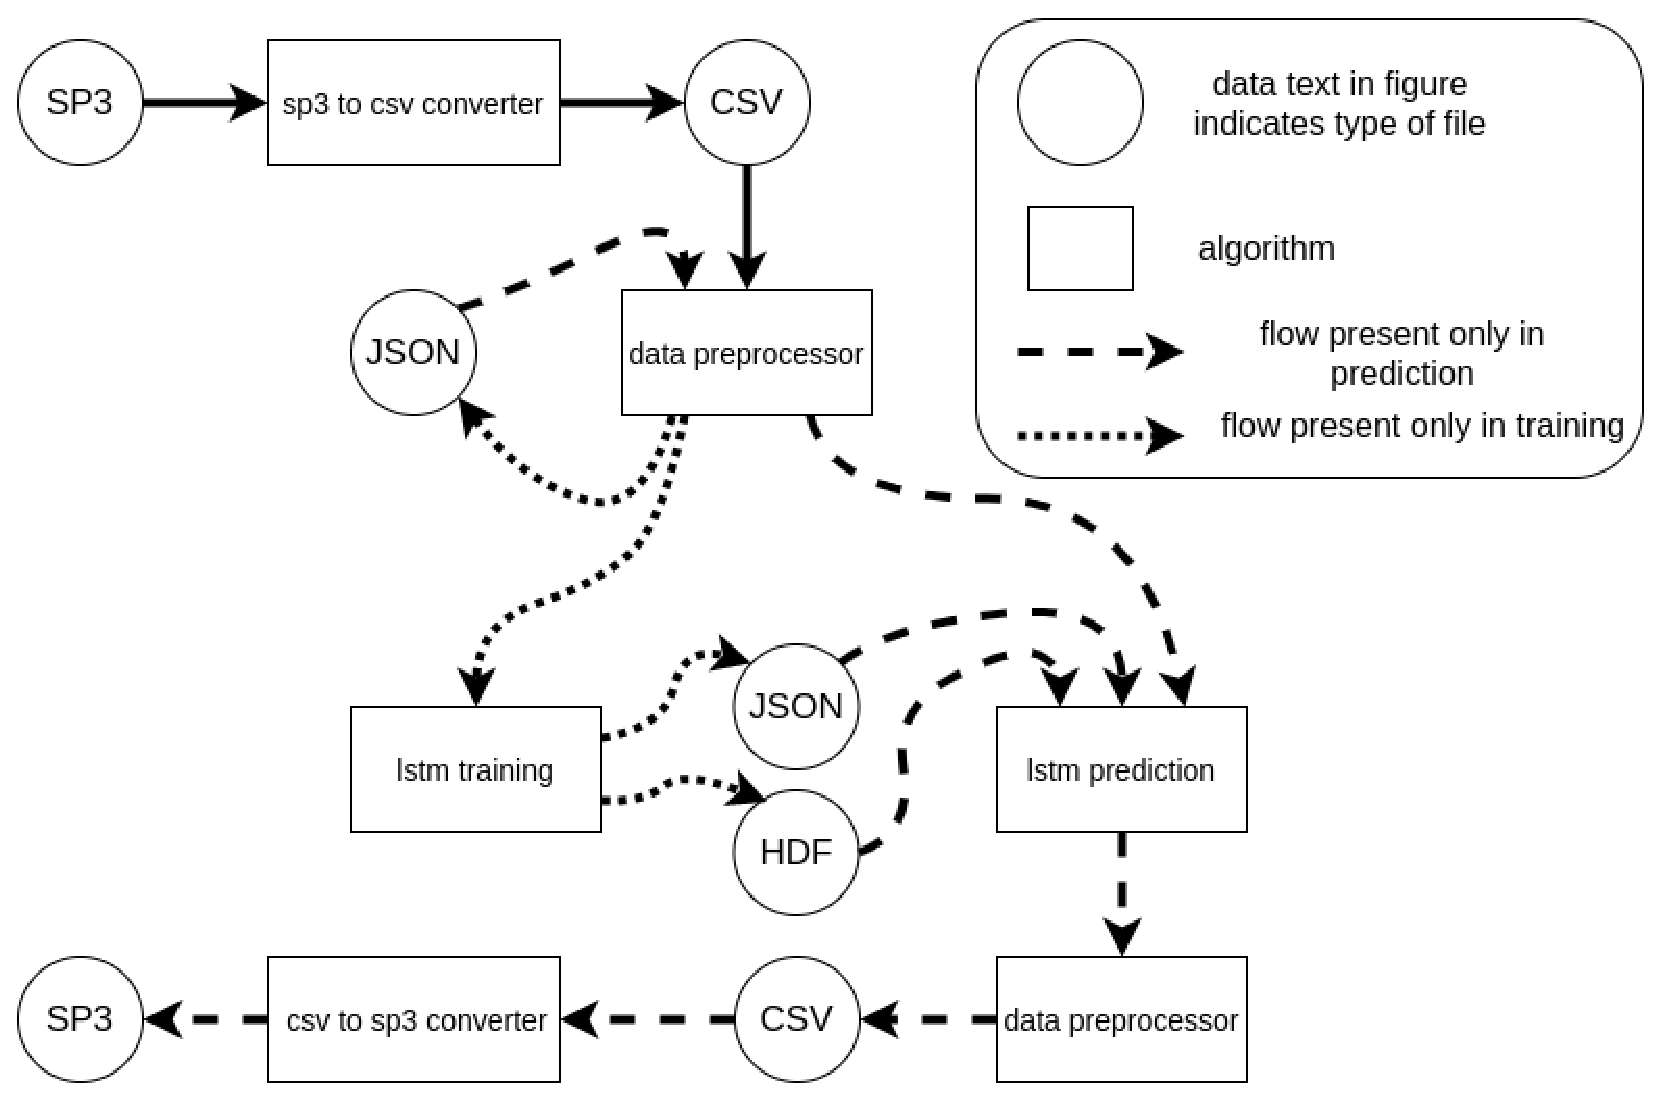
\includegraphics[width=\textwidth]{res/pipeline}
	\caption{Machine learning pipeline}
	\label{fig:pipeline}
\end{figure}
Data is received in Standard Product 3 (sp3) format that contains information about satellites
orbits as well as about their clocks.
As this is a specialized file format and is not most convenient to work with first step extracts
data from sp3 format into CSV which is a more general-purpose format.
For the next step Python script reads CSV file and stabilizes time series by differentiating it,
this is an important step as neural networks work best with stable data.
The original value of the first element in the series must be stored separately for the recreation
of the original data format. In the next step, stable data is shifted so that its median 
is at zero.
The last step that is common for all data pipelines is scaling, for best predictions in neural
networks, a value from the range of $[-1 , 1]$ should be used. While it is not possible 
to assure that no future data will fit into that range it is possible to make it less likely.
%TODO: Write more precisely how we deal with out of range values
The scale is given as an algorithm parameter and may be calculated either based on the clock model
or available data. In the case of this experiment, the largest absolute value in the test set was
used as a scaling factor.
At this moment depending on either this is a train or a prediction pipeline one of two things
will happen.
In the case of the training pipeline, data will be divided into training and evaluation
portions and the neural network will be adjusted to it. The result of this pipeline are *.hdf5 and
*.json files that store respectively weights and topology of a network.
In the case of a prediction pipeline, an already prepared weights and topology will be loaded and
series will be extended with predictions. The number of predictions depends on the prediction depth
parameter. After that time series will be returned to its original form by reverse scaling
median shift and integration.
The predicted part will be returned as a CSV file with epochs starting at the point 
in which the original data ended.
The resulting CSV can be finally converted back into an sp3 file that may be used 
for calibration of localization algorithm.

\paragraph{Data source}
For this work three of IGS provided products are used. Ultra-rapid observed is used as a
training and network input in the prediction phase. Predicted half of the same product 
is used to compare the prediction quality of LSTM.
The observed half is used as a reference bias, in other words, the bias prediction error is
the difference between the predicted value and IGU observed half.
\begin{table}[h] \label{table:2}
	\parindent0pt
	\caption{Products used in experiments}
	\centering
	\begin{tabular}{lcl}
		\hline
		\hline
		Type &Accuracy &Latency\\  
		\hline 
		Ultra-Rapid predicted half &1.4 ns &real time\\  
		Ultra-Rapid observed half &50 ps & 3-9 hours\\  
		\hline 
		\hline
	\end{tabular}
\end{table}
This data was downloaded from repositiory provided by European Space Agency\cite{ESA}
It is important to remember that the prediction system designed in this work does not intend to 
compete with long latency high accuracy products but only with those that provide 
real-time predictions.
To test the validity of LSTM as a predictor single satellite (G05) will be used.

\paragraph{Data preprocessing}
%TODO: Fix next sentence to make it more clear
IGU provides raw clock bias, this poseses two problems for the approach used in this work.
Constant clock drift is a major source of an error it suppresses other error types
as seen in figure \ref{fig:raw_bias} in visualization it makes data seams linear.
\begin{figure}[h] 
	\centering
	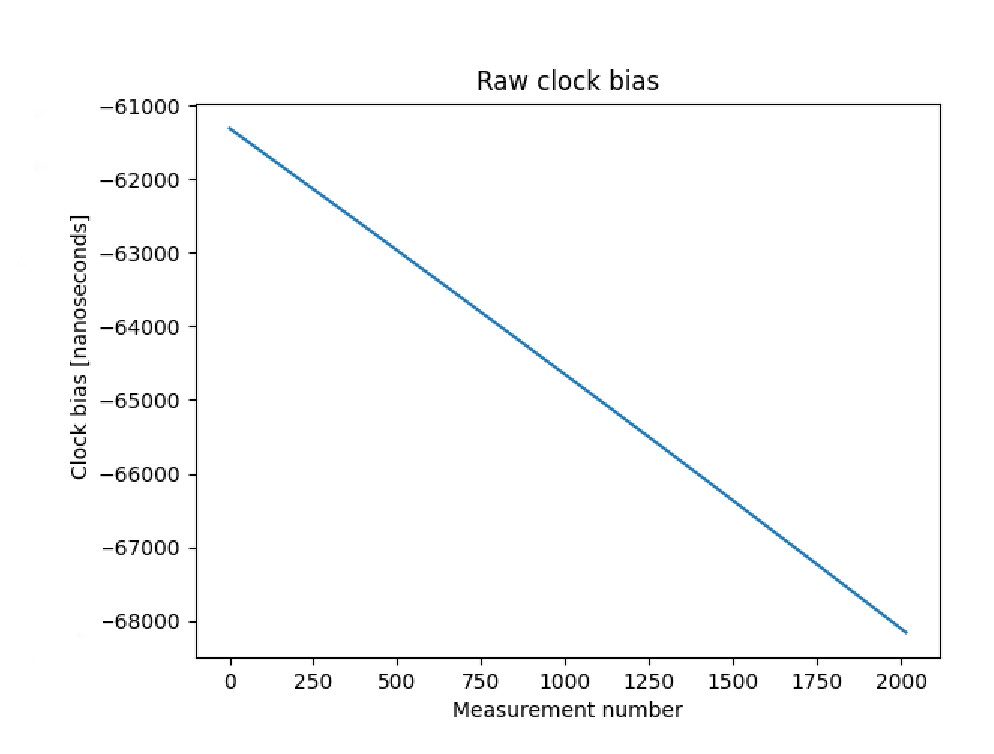
\includegraphics[width=10cm]{res/bias_raw}
	\caption{Raw clock bias}
	\label{fig:raw_bias}
\end{figure}
This trend implies the non-stationary nature of series, this is a problem as neural networks work 
best for stationary data with mean at 0 and values inbetween -1 and 1.
To solve this problems first series is differentiated which returns data where other noises 
besides constant shift are visible as seen in Figure \ref{fig:diffed_bias}.
\begin{figure}[h] 
	\centering
	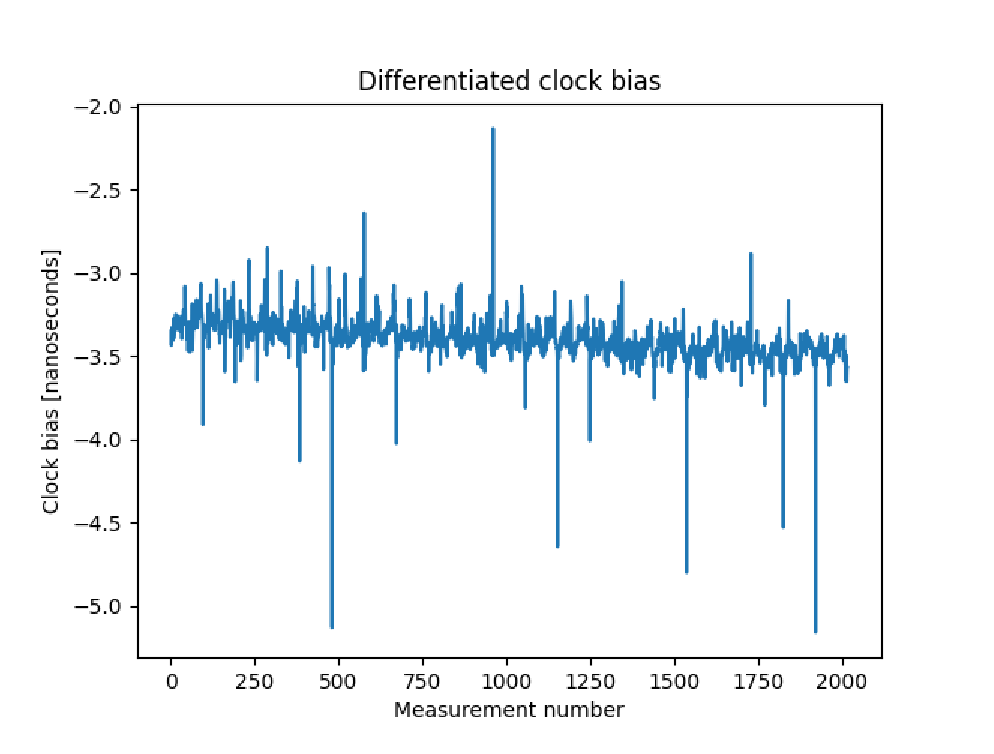
\includegraphics[width=10cm]{res/bias_diffed}
	\caption{Differentiated clock bias}
	\label{fig:diffed_bias}
\end{figure}
Constant drift is still present as a shift at the y-axis, to remove it a mean 
shift must be performed.
Finally, data must be scaled so that there will be no values with an absolute value above one.
It is, of course, possible for future prediction inputs to have absolute value above one 
however this will not be a problem as the network can deal with such inputs especially 
if they appear rarely in series.
Results of complete preprocessing of signal are visualised in Figure \ref{fig:bias_normalized}
\begin{figure}[h] 
	\centering
	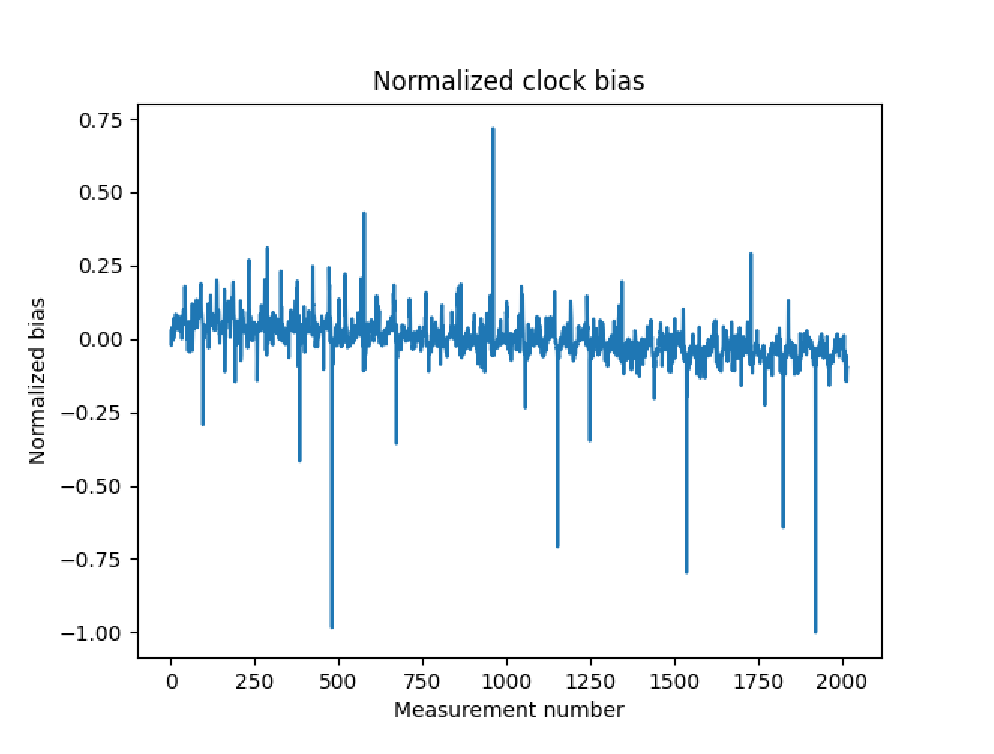
\includegraphics[width=10cm]{res/bias_normalized}
	\caption{Comparison of differentiated clock bias}
	\label{fig:bias_normalized}
\end{figure}
%----------------------------------------------------------------------------------------------------
\subsection{Phase 0 validation of approach}

%----------------------------------------------------------------------------------------------------
\subsection{Phase 1 implementation for all satellites}

%----------------------------------------------------------------------------------------------------
\subsection{Phase 2 network model updates}

%----------------------------------------------------------------------------------------------------
\subsection{Phase 3 hyperparameter adjustement}

%====================================================================================================
\section{Results}

%----------------------------------------------------------------------------------------------------
\subsection{Comparition of final results with current state of the art}

%----------------------------------------------------------------------------------------------------
\subsection{Conclusions}

%----------------------------------------------------------------------------------------------------
\subsection{Future research plans}






